\chapter{系统实现}
\label{implement}

本章节将对于上述设计的实现过程进行叙述。本章节分为三部分。第一部将介绍本系统如何基于LibISR的物体追踪系统\cite{Ren_3DV_2014, star3d_iccv_2013}实现后端服务器。第二部分将介绍本系统如何基于Unity引擎实现编著和交互系统,包括应用的游戏管理器的实现,以及应用中各个场景的具体实现。其中重点介绍编著系统对于用户需求中的各个功能的实现,以及交互场景中将服务器的物体追踪数据应用到最终的增强现实场景中的物体上的实现方法。第三部分将介绍在客户端和服务器之间进行通讯的实现。

\section{物体追踪系统的实现}
本系统基于开源物体追踪工具,LIbISR进行实现。在使用原有算法的基础上,进行了一定的修改。本系统使用的深度摄像头是Kinect第二代,但是原工具是基于第一代开发的。两代摄像头存在着一定的差异,包括驱动的支持情况、图像的分辨率等。这些因素导致了源程序并不能直接运行,本系统在开发过程中对其进行了一定的修改。

\subsection{Libfreenect 2的适配}

原系统使用openni为驱动获取Kinect数据。但是openni并不能有效获取Kinect 2的数据,并且已经停止更新和维护了。因此本系统使用了Libfreenect 2作为替代。

LibISR对于不同的硬件提供了统一的接口ImageSourceEngine。它是一个纯虚类,只需要添加新的实现,并且在初始化的时候进行修改就可以使用不同的驱动了。在实现时,保存了Private data类,将驱动的不变数据,例如device指针,listener指针,以及从相机获取的数据进行保存。实现获取图像,需要首先根据文档要求进行初始化。初始化时,软件遍历连接的USB接口获取设备,选择使用CUDA进行加速,初始化RGB、红外线发生器、深度摄像头三个设备,配置深度摄像头的范围。Libfreenct 2还自带了使用Kinect默认标定数据生成RGB-D图像的功能,经过验证也具有比较好的融合效果,但是本系统仍然使用了自己的标定数据,Libfreenect 2只提供了融合之后的图片,而缺乏中间数据。此外,Libfreenect在初始化之后没有被使用的话就会被自动关闭,但是LibISR需要在初始化图像源之后进行其他操作,因此这里创建了新的线程,在初始化之后就会进入死循环,在软件结束之后回收,保证驱动不会自动关闭。

初始化之后,程序每一帧会调用该函数获取图像。获取图像时会首先获得数据在CPU当中的指针,然后将获取到的图像进行逐一复制。LibISR中图像都是基于数组封装的,但是进行逐一复制而不是memory set的原因是,RGB图像摄像头获得的数据是BGR因此需要转换颜色通道,而深度图像摄像头获得的是32位float,而程序中实际使用的是16位short int。

转换完成后,就可以将获取的图像应用到后面的计算了。

\subsection{相机标定与RGB-D图像融合}
由于Kinect 1的彩色图像分辨率为640*480,深度图像分辨率为320*240,两者成比例,并且可以通过设置驱动直接获得相同分辨率的图片,因此源程序存在应用错误、逻辑基于两者分辨率相同的情况。但是,Kinect 2的彩色图像分辨率为1920*1080,深度图像分辨率为512*424,不成比例。因此需要在获得图像后进行融合。为了融合两个相机的图像,需要找到深度图中每个像素点对应在RGB图像中的坐标。

这一过程需要对相机标定从而获得相机参数。本项目的标定使用了基于ROS系统的iai kinect提供的标定工具\cite{iai_kinect2}。该系统通过拍摄多个角度的确定规格的棋盘格,可以计算出RGB相机和深度相机的内参,包括相机的焦距以及图像中心等。同时,通过在同一时刻获得相机的深度图像和RGB图像,可以获得相机的外参,即深度摄像机和RGB摄像机之前的位移和旋转关系。之后可以通过他们计算出坐标映射公式。

设$P_{rgb}$,$P_{ir}$分别为彩色摄像头和深度摄像头各自的相机坐标系下的一点的非齐次坐标,对应的像平面坐标分别为$p_{rgb}$,$p_{ir}$,彩色摄像头和深度摄像头的内参矩阵为分别为$H_{rgb}$和$H_{ir}$,根据相机的映射公式,可得相机坐标系与像平面的点的对应映射关系为:
\begin{equation}
 p_{ir} = H_{ir}P_{ir} \quad\mathrm{,}\quad  p_{rgb} = H_{rgb}P_{rgb}\label{camera1}
\end{equation}
由标定可以得到两个摄像机之间的外参矩阵,包括旋转矩阵R和平移向量T。则两者相机坐标系之间的对应关系为:
应映射关系为:
\begin{equation}
 P_{rgb} = RP_{ir} + T \label{camera2}
\end{equation}
将公式(\ref{camera1}),(\ref{camera2})整合,可以得到两个相机的像平面之间的点的映射关系为:
\begin{equation}
 p_{rgb} = H_{rgb}RH_{ir}^{-1}p_{ir} + H_{rgb}T
\end{equation}
由此公式就可以得到深度图像中每个点在彩色图像中的点的坐标了。为表达简便可设置
\begin{equation}
 H = H_{rgb}RH_{ir}^{-1} \quad\mathrm{,}\quad T_H = H_{rgb}T
\end{equation}

由$H$,$T_H$构成的矩阵就是单应性矩阵了,它描述的是彩色相机和深度相机的像平面之间的映射关系。由于其中的像平面坐标为三维非齐次坐标,但实际使用的时候为二维坐标,也就是三位齐次坐标,因此需要在使用时进行转换,其中三维非齐次深度坐标的z值就是该点的深度。
	
本系统在Low Level Engine中实现了融合。为了运算效率考虑,系统中将深度图映射到了彩色图,使用深度图的分辨率。融合使用了CUDA代码,首先将数据从CPU复制到GPU,并且分配所需要的线程块和线程数目。在本系统中,使用了8*8的线程块(block)结构,以及64*53的网格结构,从而实现将每个像素分配到一个线程。由于CUDA代码中每个线程运行的时候都可以获得自己的block ID和thread ID,再加上block的结构,就很方便的计算出对应的像素位置。得到像素的位置,就可以利用上述的单应性矩阵公式计算出该像素在彩色图中对应的位置了。
	
\begin{equation}
 X_{rgb} = threadID.x + blockID.x * blockDims.x
\end{equation}
\begin{equation}
 Y_{rgb} = threadID.y + blockID.y * blockDims.y
\end{equation}

这一部分函数输出了两张图,一张是融合之后的RGB-D图,其中a通道代表深度值。另一张是对齐的彩色图,它是将RGB-D图像的a通道设为1之后得到的,彩色图缩小之后可以与深度图对齐的图像。

\subsection{追踪结果显示}

由于Kinect 1中两幅图成比例,因此UIEngine可以在基于深度图大小计算出追踪结果后将其按比例放大叠加在彩色图上。但是,当二者不成比例时,追踪结果就会出现扭曲。因此这里使用了对齐之后的rgb图像作为代替。虽然这样做不会有实质的影响,但是由于对齐之后的彩色图存在硬件造成的噪声和重影,会对显示效果有一定的影响。

\section{客户端的实现}
本小节将详细介绍按照设计的架构,包括绍游戏管理器,以及应用中各场景的实现。

\subsection{游戏管理器}
游戏管理器会在基准场景(base scene)中生成,而且这个场景不会被销毁。为了保证只有一个游戏管理器,在初始化的时候使用了单例模式,GM\_Core中包含了一个静态指针,指向一各游戏管理器实例。当其他对象尝试创建新的对象的时候,会被销毁。

在每次需要切换场景的时候,游戏管理器会先将当前场景(如果有的话)进行卸载,然后启动coroutine异步加载另一个场景,该场景的加载模式为additive,表示在当前场景的基础上进行加载。加载完成之后该coroutine会进行返回,返回之后会根据新的场景中GM Settings的情况修改场景光照。如果加载过程太长的话,在这一个过程中可以添加等待场景加载的动画。

\subsection{编著场景}
编著功能主要在Build Experiment场景中进行实现,本小节将首先介绍场景中的用户接口(UI),然后根据实现需求进行相应的介绍。

\subsubsection{用户接口(UI)实现}
编著场景中实现了五个用于交互的菜单。

\begin{itemize}
    \item \textbf{Settings Menu}
用于修改实验场景。实验环境编辑需要调整光照颜色与强度,相机高度与角度,实验环境(室内或是室外)等。因此使用了滑块(Slider)和开关(Switch)等控件,并添加一个半透明panel用于和场景区分。滑块封装了OnValueChange函数,会在滑块发生移动的时候触发。相似的,开关控件会在被修改的时候调用控制函数。
    
    \item \textbf{Tool Menu}
用于添加物体。用户点击添加物体按钮后,会播放动画将选择物体类别的菜单显示出来,用户可以选择要添加的物体类别,之后软件显示所有支持物体的图片,点击对应图片就可以添加物体了。选择物体类别的菜单由UI\_List实现,目前支持“容器”、“药品”、“工具”、“预置组合”四类。UI\_List本身具备垂直布局(vertical layout),它会将子对象自动按照竖直排列。而每一个子对象对应一种物体类别,并且绑定了onclick函数。选择类别后弹出的选择具体物体的菜单由UI\_Bag实现,他也包含了一个网格布局(grid layout),会自动将子对象按照网格排列。他的子对象都是预制体(prefab),可以显示图片,并且绑定了创建物体的onclick函数。
    
    \item \textbf{Substance Menu}
用于编辑药品属性和量。其中包括,选择物质种类的下拉框(dropdown),以及输入物质的量的输入框(input field)。下拉框使用了OnValueChange函数,在选择发生变化的时候触发。输入框绑定了OnEndEdit,在编辑完成的时候触发。

    \item \textbf{Blackboard Menu}
用于编辑场景中的实验提醒文字。包括调整文字的大小和颜色,设置与settings menu类似。
    
    \item \textbf{Step Menu}
用于设置实验的步骤等信息。最上方设置了输入实验名称的输入框。一侧使用了vertical layout显示当前的已有的流程,另一侧显示当前已有的步骤。这里的流程和步骤都使用了同一个预置体。中间提供了输入流程名称、步骤名称的输入框,以及选择对应事件的下拉框。他们都绑定了对应的OnValueChange函数,在获得用户输入的时候触发。
\end{itemize}
~\\
\indent    	这些菜单会通过场景中的按钮或用户输入触发,同时会暂停触发场景其他交互行为,防止在用户调整菜单的时候出现干扰。在菜单之下还会生成一个覆盖整个屏幕的透明按钮,实现当用户点击的时候关闭菜单,并且确定用户输入输入,恢复场景其他交互。

\subsubsection{实验场景编辑}
当用户点击场景编辑按钮后,会弹出编辑场景的菜单(Settings Menu)。当用户移动其中的滑块时,会触发OnValueChange函数,调用控制Slider的引擎,UI\_Slider,它保存了场景中相机、光源的指针,会读取此时slider的值,并且修改对应物体的属性值。如果通过开关调整实验环境,开关的控制器会修改对应的场景模型。

\begin{figure}[!htp]
  \centering
  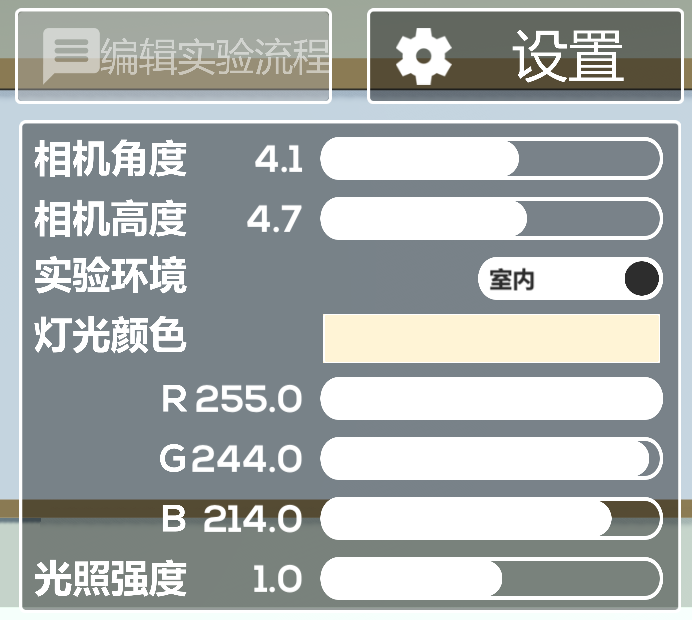
\includegraphics[width=8cm]{figure/settings.png}
  \bicaption[实验场景编辑用户接口截图]
    {实验场景编辑用户接口截图}
    {The Screenshot of Experiment Editing UI}
 \label{fig:gm}
\end{figure}

\subsubsection{物体编辑}
场景中的物体首先通过菜单进行添加。支持物体以及他们的种类通过静态二维链表储存。

	当用户选择添加物体之后,选择物体种类的菜单弹出(Tool Menu)。物体种类被选择后,控制器UI\_List会查找二维链表,获得对应类别的物体图片,并创建显示该图片的预制体,添加到选择物体的菜单中。用户选择物体之后,会通过对应物体的名字,在资源文件夹中查找对应的预制体游戏对象,添加到场景中,完成物体创建。
	
\begin{figure}[!htp]
  \centering
  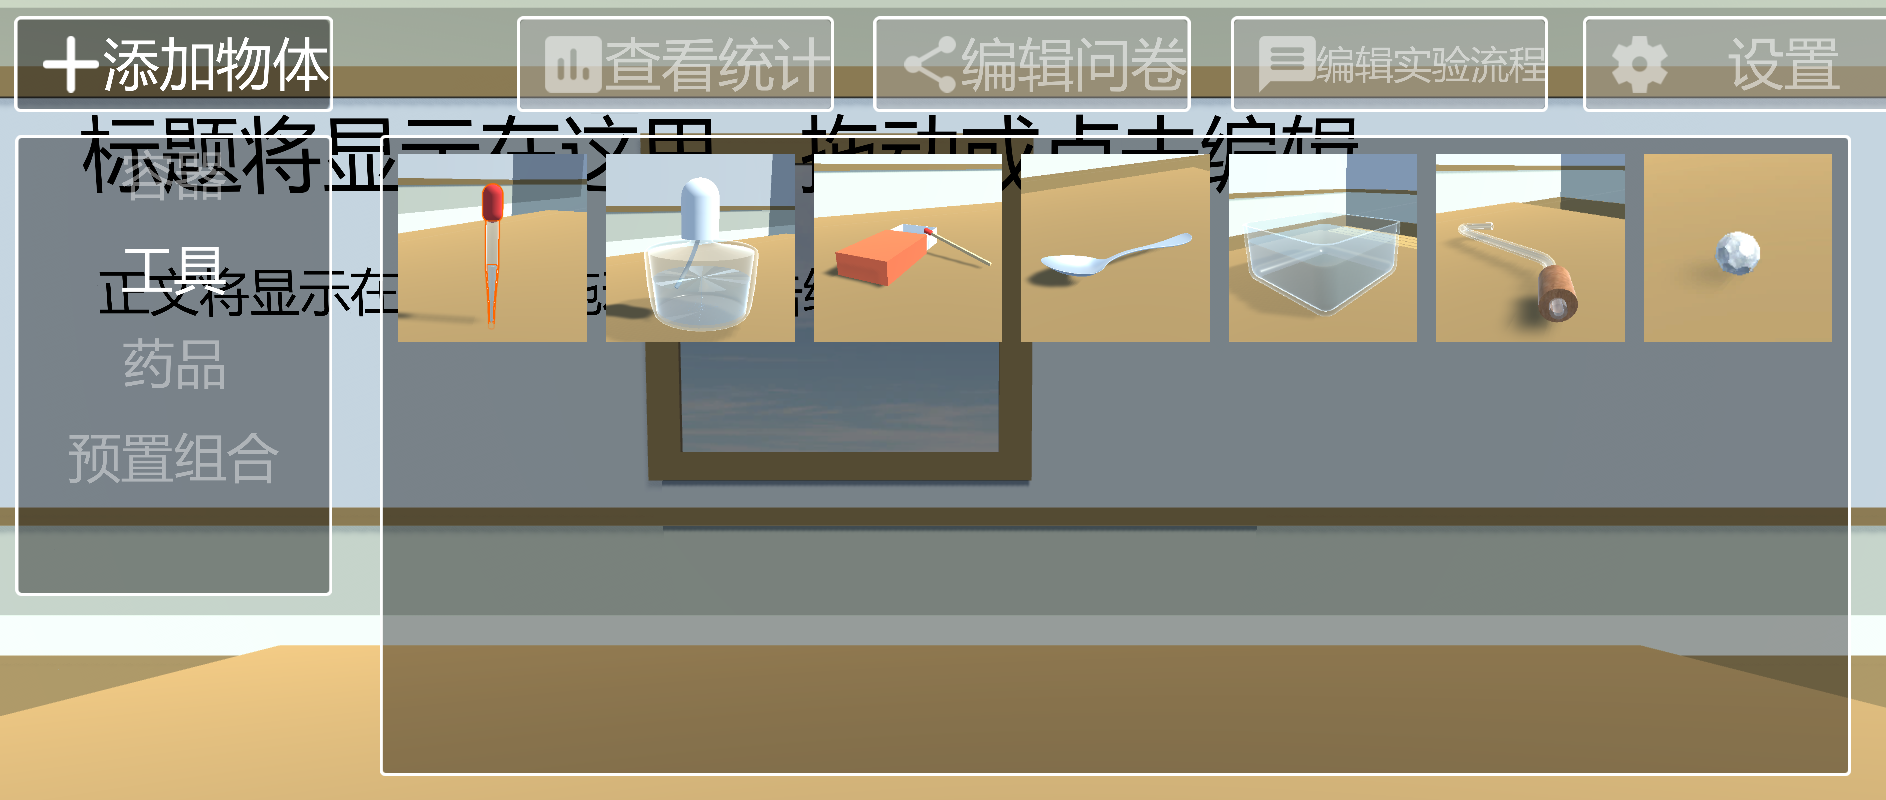
\includegraphics[width=12cm]{figure/addObj.png}
  \bicaption[添加物体用户接口截图]
    {添加物体用户接口截图}
    {The Screenshot of Adding Object UI}
 \label{fig:gm}
\end{figure}

	创建好的物体通过控制器Lab\_Controller进行控制。Lab\_Controller会在用户触发点击事件的时候,从相机位置向点击位置发出一条射线,之后获取射线碰撞的第一个物体。同时,控制器会在每一帧计算距离用户点击时刻的时长,如果在到达一定的阈值之前检测用户松开鼠标,则触发单击对应的事件。如果超时,则会判断用户触发拖动事件。

	如果是单击事件,首先判断接触到的是否是可以编辑的物质,判断的方式是该物体是否具有container类,该类用于保存物体包含的物质的种类和量。如果有,则将编辑物质的菜单(Substance Menu)进行显示。下拉框会在初始化的时候获取所支持的物质,并且修改选项。为了保证物质的量为浮点数,需要对输入框的格式进行设置。完成编辑后,控制器会将对应的用户输入赋值到该物体的container对象中。如果没有,则无效果。
	
\begin{figure}[!htp]
  \centering
  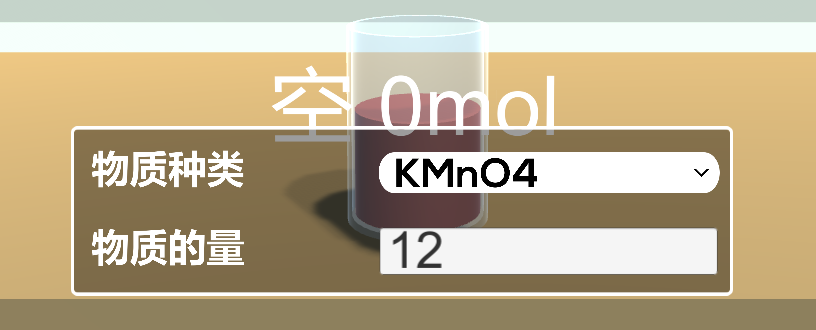
\includegraphics[width=12cm]{figure/subs.png}
  \bicaption[编辑物体种类用户接口截图]
    {编辑物体种类用户接口截图}
    {The Screenshot of Editing Object UI}
 \label{fig:subs}
\end{figure}

编辑好的物体会将物质信息显示在模型外,效果见图\ref{fig:subs}和\ref{fig:substi}。显示的文字通过3D Text实现,会在修改之后触发相应的函数修改其text mesh的内容。

如果是拖动事件,依然首先判断物体是否是可以移动的物体,所有添加的物体都是可以移动的,他们使用Object的标签进行标记。这里的目的是避免拖动桌子、墙壁等其他静态物体。之后会在每一帧由相机向点击位置发出射线,将当前拖动的物体放置在射线和碰撞体的交点上。此时需要先去除拖动物体的碰撞体,否则物体会沿着射线方向一直向相机移动。当用户松手的时候,物体就会停留在最后移动的位置,并且恢复物体的碰撞体保证可以进行下一次移动。

由于一些实验中往往需要流程化的实验步骤,例如产生气体之后通入水槽等,需要气体发生装置和收集装置相对位置固定,因此添加了UI\_Anchor进行引导。UI\_Anchor是与桌面平行的平面碰撞体,当上述的交点接触到锚点(anchor)时(同样使用tag进行标记),会在锚点中心生成一个目前拖动物体的复制,并且修改它的材质为半透明单色,并把该物体的指针赋给UI\_Anchor中的对应变量。如果此时用户松开鼠标,则拖动中的物体就会代替复制,被固定在锚点上。当用户需要将物体从锚点移开的时候,则会制造先出复制,直到点击位置离开锚点范围之后删除复制,在这过程中如果用户松开鼠标,则物体会返回锚点处。。
	
\begin{figure}[!htp]
  \centering
  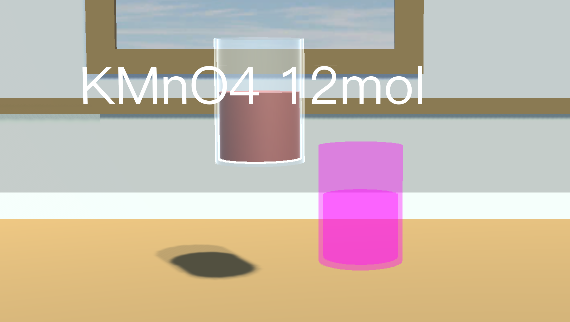
\includegraphics[width=8cm]{figure/substi.png}
  \bicaption[锚点物体复制效果图]
    {锚点物体复制效果图}
    {The Effects of Objects Substitution on Anchor}
 \label{fig:substi}
\end{figure}

场景中有多个平行锚点,它们都在同一个实验桌上,由UI\_Table控制。UI\_Table会储存桌子上的锚点的物体信息,并且在鼠标移入、移出锚点,即真正添加和删除物体的时候,根据所有锚点的位置和占用情况,对其余物体进行移动操作。如果在添加的时候发现所有的锚点都被占用,则不会创建新的复制,物体也不能被移入锚点。

基于上述机制,物体在创建的时候会优先创建在锚点上。只有当物体太多、锚点都被占用的时候,才会被创建在桌面上的其他位置。综上所述,物体的创建、移动、内容编辑就实现了。


\subsubsection{提示信息编辑}
实验过程中需要显示实验名称,并且对用户进行实验步骤提示,用户可以通过编著系统修改该提示信息的位置、大小、颜色等属性。

\begin{figure}[!htp]
  \centering
  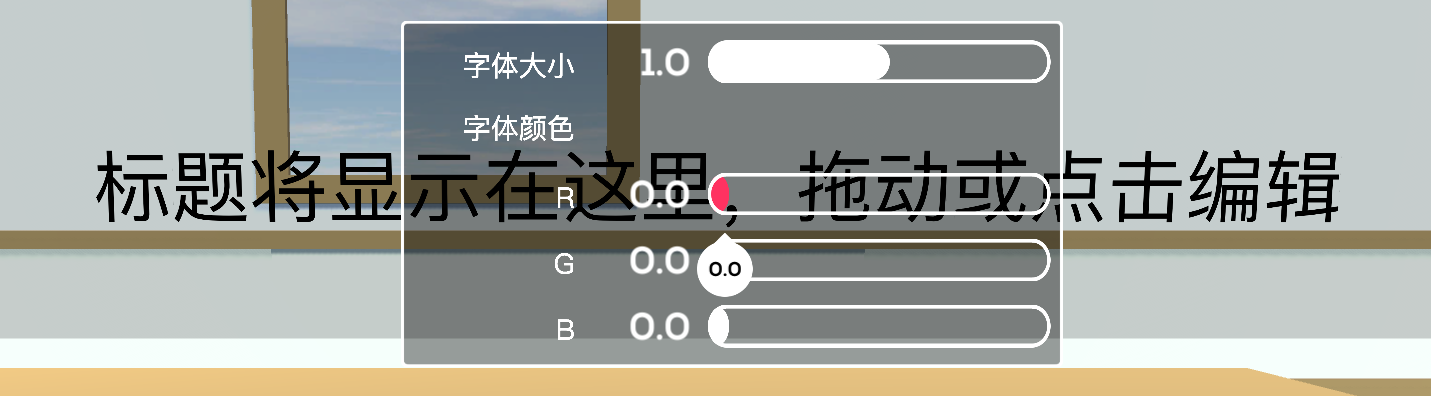
\includegraphics[width=12cm]{figure/text.png}
  \bicaption[编辑提示文字外观用户接口截图]
    {编辑提示文字外观用户接口截图}
    {The Screenshot of Editing Hints Appearance  UI}
 \label{fig:gm}
\end{figure}

用户可以编辑提示文字的显示方式。在lab controller获取到点击事件之后,如果点击的物体标签为text,则会首先获得物体中的text对象,用其中的属性值,包括字体的颜色、大小,初始化字体编辑的页面的控件的值,然后显示该菜单。用户在编辑之后,相应的文字就会被修改并立即显示了,编辑完成后,还会修改字体的text对象内的变量值,保证下一次操作的正确性。。

当用户触发长按事件,则按照与移动物体相似的逻辑移动字体,只不过在移动物体的时候如果点击位置不在字体可显示范围之内,文字就不会再发生移动。由于这些文字需要在三维场景中移动,因此也使用了3D Text。但是3D Text默认情况下会永远显示在最前面,如果需要其具有深度关系,需要修改使用的着色器。起初,系统自定义了新的着色器,但是,修改之后的着色器只能通过修改材质中的颜色参数才能修改颜色,修改text mesh的颜色是无效的,这在一些使用场景下(如WebGL)下是不被支持的。此外,需要的着色器会使文字在一定位置显示特殊的反射。最简单有效的方法,是将3D text的着色器修改为一般的2D字体的着色器,然后使用中文字体。

\subsubsection{实验流程编辑}
用户也可以通过编著系统,编辑用户在进行实验时参考的提示信息内容。

\begin{figure}[!htp]
  \centering
  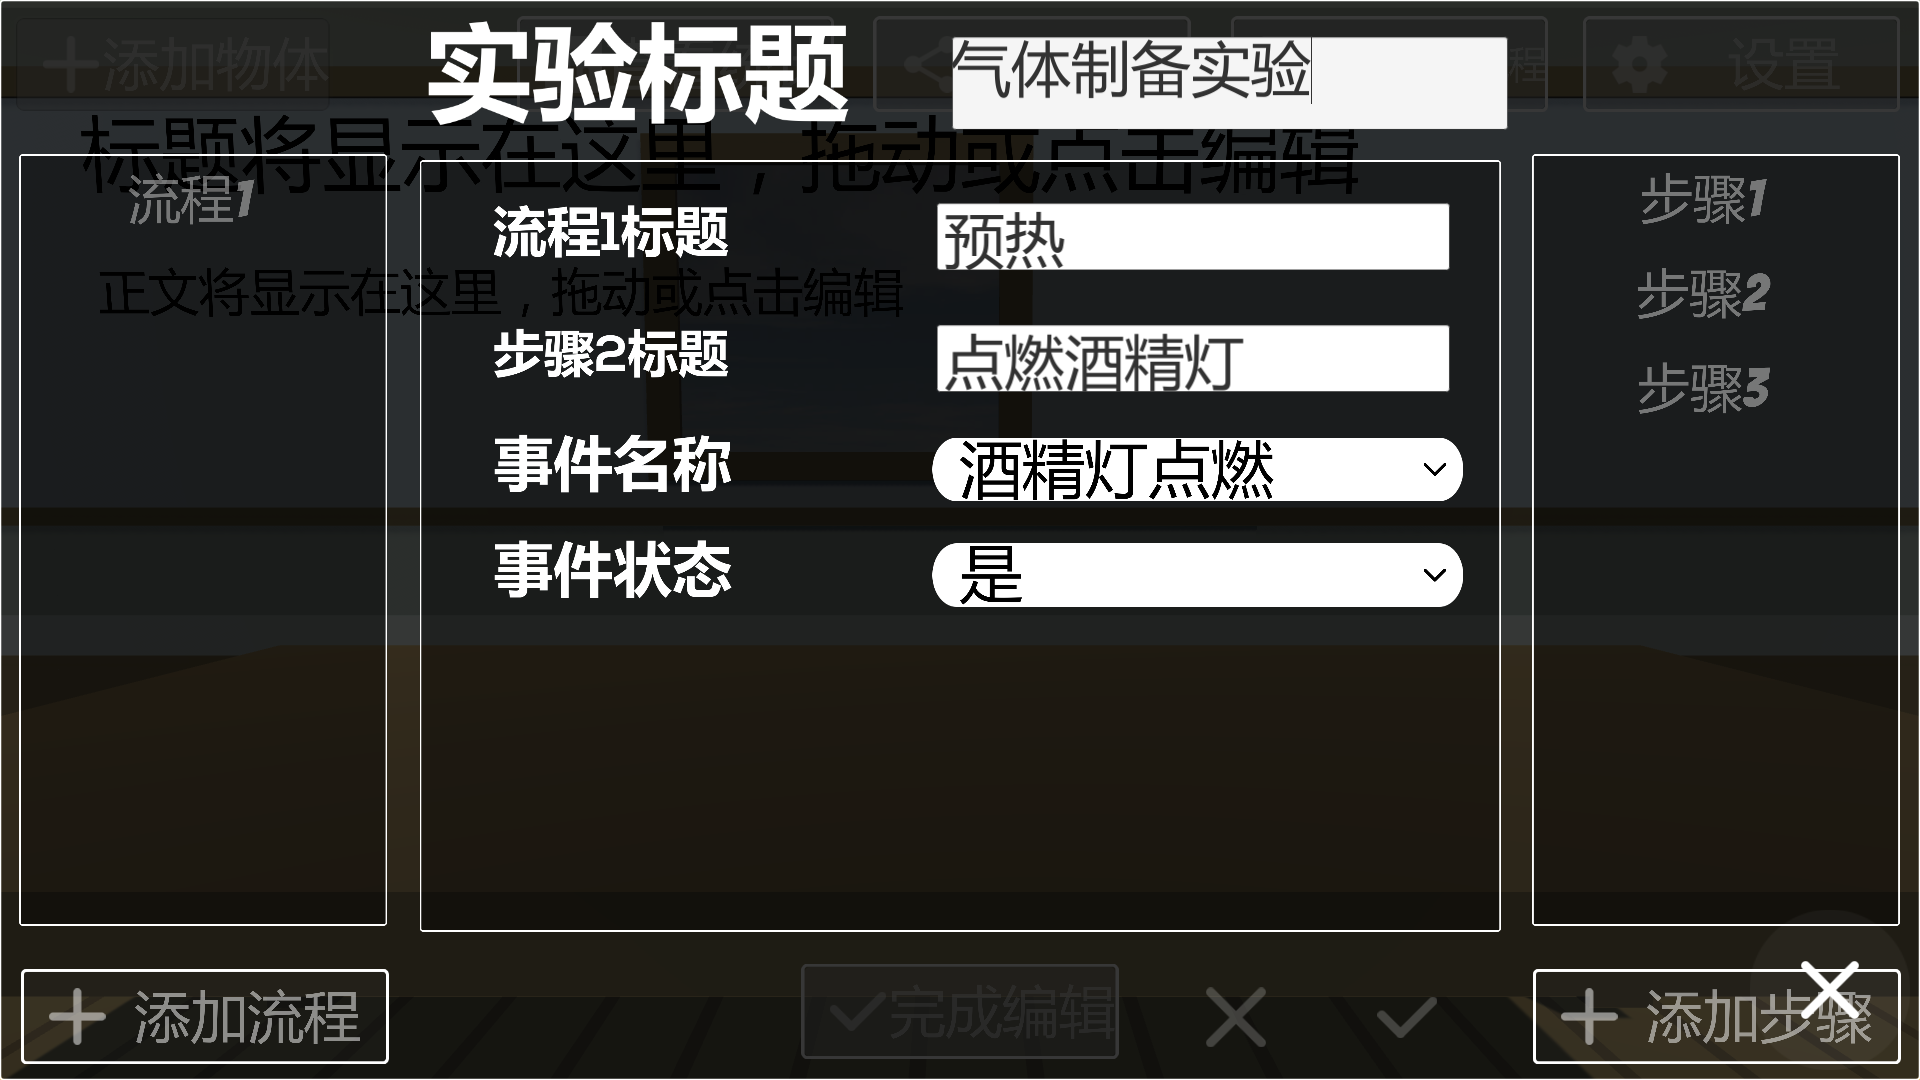
\includegraphics[width=12cm]{figure/step.png}
  \bicaption[编辑实验流程用户接口截图]
    {编辑实验流程用户接口截图}
    {The Screenshot of Editing Experiment Procedure UI}
 \label{fig:gm}
\end{figure}

当用户选择实验流程编辑的时候,会显示对应的菜单。用户首先可以添加流程,流程由预制体构成,添加的流程将会追加在显示流程的滑动框(scroll content)的子对象中,并且自动按照vertical layout进行排列。点击一个创建的流程之后可以为它添加对应的步骤,步骤使用同样的预制体实现,并使用布尔值进行区分。添加的步骤会追加在显示步骤的滑动框的子对象中。流程、步骤都可以通过输入框修改名称,步骤还需要设置对应的操作事件,可用的操作事件会在初始化的时候向游戏管理器发出请求获取,并且通过下拉框供用户选择。关于步骤、流程的上述属性都会在发生修改之后,保存在各自的step对象中。

实现过程中发现,文字输入框会产生一些中文文字不能输入的情况,这是由旧版Unity产生的bug,需要更新Unity版本进行解决。

编辑信息由UI\_Step进行控制。他保存了一个记录所有流程的指针数组,以及记录每个流程对应步骤的二维指针数组。UI\_Step还记录了当前的流程和步骤序号,当用户切换步骤的时候,会读取当前的step中的信息,并且把对应数据显示在控件上。当用户切换流程的时候,会从二维指针数组中激活对应的步骤,而将当前显示的步骤隐去。


\subsubsection{编辑已有实验}
用户可以将已经编辑的实验进行保存,并且在下一次使用的时候继续编辑。

用户需要首先将当前的编辑内容全部保存下来。负责该功能的是UI\_Edit。他会在用户保存编辑内容的时候,将场景数据保存在游戏管理器的experiment setup对象中,其结构见图\ref{fig:uml},并且通过网络发送数据,保存在数据库。其中场景的编辑数据通过编辑菜单获得,场景中的提示信息属性通过场景中的两个文字对象的相关属性获得。所有的物体创建后都会成为object list的子对象,遍历object list可以获得所有创建物体的相关属性。而实验流程则通过保存在UI\_Step中的两个列表获得。

将上述变量保存之后,在编辑已有场景的时候,场景会在初始化的时候从游戏管理器读取该对象,将所有属性还原。其中场景的还原,包括将还原的数据作用于场景中的对象上,并且修改场景编辑菜单控件的初始值。提示文字按照数据修改相应的颜色、位置等数值。物体的还原需要按照物体的名字、物质的量等信息,重新初始化游戏对象,仍然添加在object list下。步骤的还原需要按照数据,还原出所有的流程、步骤按键,并且放置在对应的滑动框的子对象下,还需要还原UI\_Step中的记录所有流程的指针数组,和记录每个流程下的步骤的二维指针数组。之后场景的还原就完成了,用户可以在此基础上继续编辑实验。

\subsection{交互场景}
交互场景中主要实现了利用追踪数据还原在Unity中的物体的姿态信息、使用Vuforia实现二维码识别,将虚拟物体与手机画面中的真实物体融合三部分。

\subsubsection{追踪结果还原}

交互场景中,需要将物体追踪服务器计算出的物体姿态进行还原。物体的姿态用一个由旋转矩阵和位移向量构成的4x4矩阵表示,其中的旋转矩阵位于矩阵左上角,可表示为
\begin{equation} 
R = 
 \begin{Bmatrix}
   m00 & m01 & m02 \\
   m10 & m11 & m12 \\
   m20 & m21 & m22  
  \end{Bmatrix}
\end{equation} 
  其中的T可以直接对应Unity场景中的位置。但是旋转矩阵则需要通过计算转换为Unity中表示旋转的四元数格式。旋转矩阵描述的是,一个向量绕单位轴$N(n_x, n_y, n_z)$旋转$\alpha$的旋转变换。公式表示为
  \begin{equation}\label{R1}
 R = 
  \begin{Bmatrix}
   n_x^2(1-cos\alpha)+cos\alpha & n_x n_y(1-cos\alpha) - n_zsin\alpha & n_x n_z(1-cos\alpha) + n_ysin\alpha \\
   n_x n_y(1-cos\alpha) + n_zsin\alpha & n_y^2(1-cos\alpha) + cos\alpha & n_y n_z(1-cos\alpha) - n_xsin\alpha \\
   n_x n_z(1-cos\alpha) - n_ysin\alpha & n_y n_z(1-cos\alpha) + n_xsin\alpha & n_z^2(1-cos\alpha) + cos\alpha 
  \end{Bmatrix}
\end{equation}
而同样的旋转可以用四元数进行表示,即
  \begin{equation}\label{R2}
Q(w, x, y, z) = [cos(\alpha/2), (sin(\alpha/2)n_x, sin(\alpha/2)n_y, sin(\alpha/2)n_z]
\end{equation}
将公式(\ref{R2})通过三角倍角公式带入公式(\ref{R1})可得
  \begin{equation}\label{R3}
 R = 
  \begin{Bmatrix}
   1-2y^2-2z^2 & 2xy-2zw & 2xz+2yw \\
   2xy+2zw & 1-2x^2-2z^2 & 2yz - 2xw \\
   2xz - 2yw & 2yz + 2xw & 1-2x^2-2y^2
  \end{Bmatrix}
\end{equation}
将公式(\ref{R3})的对角线进行加减运算,可以得到四个等式
\begin{equation}\label{R4}
\left\{
\begin{aligned}
m00 + m11 + m22 &=& 4w^2 - 1 \\
m00 - m11 - m22 &=& 4x^2 - 1 \\
-m00 + m11 - m22 &=& 4y^2 - 1 \\
-m00 - m11 + m22 &=& 4z^2 - 1 
\end{aligned}
\right.
\end{equation}
此外,还可以得到
\begin{equation}\label{R5}
\left\{
\begin{aligned}
m01 + m10 &=& 4xy  \quad\mathrm{,}\quad m01 - m10 &=& 4wz \\
m20 + m02 &=& 4xz  \quad\mathrm{,}\quad m20 - m02 &=& 4wy \\
m12 + m21 &=& 4yz  \quad\mathrm{,}\quad m12 - m21 &=& 4wx 
\end{aligned}
\right.
\end{equation}
由于四元数整体的正负是没有区别的,因此解公式(\ref{R4})取正值,带入公式(\ref{R5})可得四组解
\begin{equation}\label{R6}
\left\{
\begin{aligned}
w=\frac{\sqrt{m00 + m11 + m22 + 1}}{2} \quad\mathrm{,}\quad x = \frac{m12 - m21}{4w} \quad\mathrm{,}\quad y = \frac{m20 - m02}{4w} \quad\mathrm{,}\quad z = \frac{m01 - m10}{4w}\\
x=\frac{\sqrt{m00 - m11 - m22 + 1}}{2} \quad\mathrm{,}\quad w = \frac{m12 - m21}{4x} \quad\mathrm{,}\quad y = \frac{m01 + m10}{4x} \quad\mathrm{,}\quad z = \frac{m20 + m02}{4x}\\
y=\frac{\sqrt{-m00 + m11 - m22 + 1}}{2} \quad\mathrm{,}\quad w = \frac{m20 - m02}{4y} \quad\mathrm{,}\quad x = \frac{m01 + m10}{4y} \quad\mathrm{,}\quad z = \frac{m12 + m21}{4y}\\
z=\frac{\sqrt{-m00 - m11 + m22 + 1}}{2} \quad\mathrm{,}\quad w = \frac{m01 - m10}{4z} \quad\mathrm{,}\quad x = \frac{m20 + m02}{4z} \quad\mathrm{,}\quad y = \frac{m12 + m21}{4z}
\end{aligned}
\right.
\end{equation}
这四组解每一组的第一个值都可以作为最终结果的w值。但是,由于w太小的时候做分母会产生姿态不稳定的情况\cite{akenine2018real},因此这里实现的时候选择了四组解中w最大的一组,作为最终解。利用上述得到的四元数,可以直接在Unity引擎中应用到物体的旋转上,再将矩阵中的位移参数应用到物体的位置数据上,就可以实现将传入的矩阵应用到虚拟场景中的物体了。

\subsubsection{二维码识别}
在相关技术中提到,二维码具有对比度高、重复率低的特点,适合作为平面图片识别。

识别需要首先获得Vuforia的许可,然后将使用的图片上传到数据库,下载生成的unity package,导入到Unity场景中,并且在场景中配置权限识别码,以及匹配追踪的数据库和对应图片。然后将image target对象添加到场景中,就可以实现二维码的识别了。

设置标志的时候需要获得图片的真实大小。这里需要将图片打印出来之后测量真实长度。但是,当图片太小的时候会发生识别效果差的情况,因此需要使用比较大的二维码。

\subsubsection{虚实融合}
Vuforia识别结果会应用在场景中的image target对象中,所有需要在增强现实场景中显示的物体都需要在它的子对象中。由于物体在初始的追踪场景中与水平面就存在90度的倾角,因此在Unity场景中的物体初始化与水平面平行,倾角为0,这样才能保证二者在运行后保持相对一致。因为需要永久保持这90度的差距,因此将该物体Object设置为Image Target的一个空子对象Empty Target的子对象,并且与该对象保持90度夹角。

物体追踪的结果会应用在Empty Target上。这里需要将物体在LibISR的物体坐标系下的物体,转到Unity场景中的坐标系,再转到识别图片image target的坐标系下。保持二维码在真实场景中固定可以使得二维码的坐标系和unity坐标系保持一致。由于不确定LibISR的坐标系左右手,以及旋转轴的设置情况,因此很难通过理论确定坐标轴的转换关系,这里简单地通过观察进行解决。首先保持二维码在Unity中的的x,y,z三个方向,所在直线分别与Kinect的相机坐标系保持平行,然后通过旋转被追踪的物体,观察追踪结果在Unity中的场景的显示情况与旋转的关系,修改对应角度的正负关系,得到了正确的角度对应关系。同理,可以得到位移的对应正负关系。将计算结果应用到物体上的时候,需要修改Empty Target的相关属性。为了避免旋转相机的时候,追踪物体不相对于二维码静止,在修改它的姿态属性的时候必须修改local变量,即相对于其父对象的值。

最后,为了保证虚拟物体与真实物体能够重合,同时与二维码保持一定的距离避免手在交互的时候遮挡二维码,需要通过改变虚拟物体与二维码之间的相对位置,实现融合。此外,由于LibISR中的长度单位与Unity中不相同,因此还需要对位移进行比例调整。这些都涉及详细的参数调整。

为了方便在手机应用当中进行如上标定,在手机追踪场景中添加了一些滑块控件。滑块可以分别控制虚拟物体相对于二维码的x,y,z三个方向的偏移,以及虚拟物体的位移与真实物体之间的比例系数,还有虚拟物体的大小缩放系数。通过调整上述滑块,可以修改对应的变量,数值会显示在场景中的文本控件上。由于单个虚拟物体在摄像机画面中进行覆盖的时候,用户不能准确判断虚拟物体的深度,因此在虚拟场景中还加入了一个半透明平面,用来辅助标定。当虚拟物体可以和真实物体在移动、旋转过程中都保持融合之后,记录参数,完成标定。

完成标定之后,系统会在每次获得物体姿态信息之后,首先通过添加正负号修改位移和旋转轴,然后将位移乘一定的系数,最后加上和二维码的偏移,就可以实现虚实融合了。由于每次使用的时候二维码和Kinect的相对位置都会发生改变,因此应用中也将上述控件进行了保留。

\subsection{其他场景}

    除了上述场景之外,还实现了主页面。主页有三个按钮,分别用于创建新的实验、编辑已有实验、进入交互场景。对应的按钮在点击的时候向游戏管理器发送请求转换场景。此外,还实现了登陆和注册页面。页面都通过输入框获取用户输入,其中密码使用密码类型的输入框,会自动将用户输入用“*”代替。而注册时需要提供邮箱,邮箱限制为邮件格式的输入。如果出现输出错误,例如注册的账户名错误,登陆信息错误,则会调用场景中的错误提示模块的播放动画,进行用户提示并且播放提示音效。

\subsection{应用发布}

    应用实现之后,通过Unity进行构建(Build),产生电脑端和安卓移动端两个版本。在构建期间有一些问题需要解决。
    
\subsubsection{分辨率适配}

    在用户接口(UI)开发完成后,在不同的平台或是分辨率下会出现错位、重叠等问题,因此需要实现分辨率的自适应。首先将游戏窗口设置为16:9,该分辨率是目前比较多的显示方式。然后将放置用户接口的画布(canvas)的缩放模式设置为随屏幕大小缩放(scale with screen size),这样当分辨率在保持16:9的前提下进行大小缩放,所有的UI控件都会进行同比例的缩放,保证显示正确。最后,需要设置所有控件的锚点,即确定所有控件缩放的原点。此外,锚点也可以设置为一个区域,这样可以保证控件相对于全部屏幕的范围的比例是不变的。
    
\subsubsection{发布设置}

    项目发布前还需要对构建的场景以及他们的运行顺序进行设置,这里将所有用到的场景都添加到了列表中,并且保证存放游戏管理器的基准场景优先级是最高的,即最优先运行。
    
    在运行之后,发现一些物体的材质并没有正常显示。这是因为Unity在构建的过程中会自动优化掉没有明确使用的着色器,因此需要使用的着色器需要在构建的时候添加到需要编译的着色器列表中。
    
    此外,还发现获取所有支持的物质并且显示的下拉框没有获取到正确的物体列表,而显示了默认的选项。这是因为原本代码是在场景创建之初,通过场景中的start函数获取支持物质的列表并修改下拉框。但是构建前后场景中各个游戏对象的初始化函数的运行先后顺序是不能确定的,因此有可能下拉框列表先被修改之后,在该对象初始化的时候又将默认的选项覆盖了上去。因此只能在控件被激活时由自己向游戏控制器发出请求获取物质列表。
    
\section{网络通信实现}

本系统以c++代码实现的物体追踪系统作为服务器,用户的编著和交互系统作为客户端。

首先在服务器communication类中实现了服务器的相关代码。它会在程序开始运行的时候创建socket,设置开放的端口,并且监听该端口。然后通过创建新的线程,运行accept函数,等待客户端的链接。这会阻塞当前的线程。此外,服务器还实现了事件类,在获取到指定事件后运行事件的响应函数。服务器的线程具有一个事件对象,处理UI事件的UIEngine中保存了它的指针,并且在初始化的时候将UIEngine中实现的的事件响应函数指针绑定到该事件上。

之后在客户端的PB\_TCP中实现了客户端的逻辑,通过服务器的ip和端口进行连接,然后创建新的线程,连接服务器的socket,然后开始死循环等待服务器的数据。

当用户在交互场景中发送指令之后,客户端会调用相应的函数,将储存在PB\_Msg中的指令(command)数据结构序列化之后,向服务器发送。指令包括开始录制、开始追踪、停止追踪三种,用整形的ID表示。服务器线程接收到指令之后,首先按照指定的关键字格式反序列化,根据指令ID触发相应的事件,并发送信号。UIEngine接受到信号后,会调用相应的事件处理函数。由于程序中本身已经实现了基于glut的键盘事件响应函数,因此只需要在收到指令之后,模拟对应的键盘输入对应的事件,修改主循环的分支条件就可以了。同时,为了保证用户先启动相机,再开始追踪物体,因此对于用户输入的指令顺序也进行了判断,错误的指令并不会影响程序的运行。

当服务器开始追踪之后,会在每帧获得姿态数据,将追踪结果序列化,作为浮点数数组发回到客户端。客户端由于使用C\#代码实现,因此并不需要触发事件,直接反序列化之后,调用在PB\_Interface中实现的相应函数就可以了。但是,如果服务器连续发送多次追踪结果,而客户端只读取一次的话,会发生多个包被合成一个处理的粘包情况。因此,服务器在每次发送数据之后,都会调用recv函数,等待客户端的反馈。客户端会在接收数据之后向服务发送一个ID为-1的指令(Command),意味着收到了数据,并且陷入等待。服务器在接收到之后才会发送下一个追踪结果。但是,由于服务器不断在生成追踪数据,并且每一次都会调用发送信息的函数,为了保证每次发送的数据都是最新的,需要使用一个布尔值标记服务器现在是否可以发送新的数据,如果服务器正在等待客户端的反馈则不会更新要发送的数据,否则则更新。这会使服务器将等待客户端响应过程中产生的数据舍弃。同时,为了防止相同数据被多次发送,服务器也只会在追踪结果更新之后才发送。二者使用同一个布尔值进行标记。这样的逻辑实际上使得物体追踪的帧数和网络传输效率保持了一致,也使服务器和客户端之间互发消息的频率保持一致。

\section{本章小结}
本章节针对设计中的三个部件的实现进行了阐述。对于服务器,在原有项目的基础上,通过修改硬件驱动,进行RGB-D图像融合,以及其他工作,完成适配。对于客户端,则着重介绍了Unity引擎下各个场景的每个控件和用户接口的实现,包括它们的内部实现逻辑,以及管理它们的游戏管理器的实现。最后对于网络则重点介绍了在不同语言和职能下网络通讯的实现。
